\documentclass[11pt]{article}
\usepackage{fullpage}
\usepackage{amsthm}
\usepackage{amsmath} \usepackage{amssymb}
\usepackage{graphicx}

\graphicspath{ {./imgs/} }

\setlength{\parindent}{0pt}

\title{Introduction to Machine Learning (CO395)}
\author{Michael Tsang}

\newtheorem{defn}{Definition}
\newtheorem{eg}{Example}
\newtheorem{theo}{Theorem}
\newtheorem{lem}{Lemma}

\begin{document}

\maketitle
\section{Machine Learning}
\textit{The field of machine learning is concerned with the question of how to construct computer programs that automatically improve with experience.}

\subsection{Supervised Learning}
Learning an unknown mapping $f(x_i) = y_i$ from training data, given in the form of input  and output pairs $D = \{ (x_i, y_i) \}^N_{i = 1}$.
\begin{itemize}
  \item $D$ is the \textbf{training set}, $N$ is the number of training examples/samples/data points. 
  \item The $x_i$ are in the \textbf{feature space} $\mathcal{X}$ and the $y_i \in \mathcal{Y}$ are in the \textbf{label space}.
  \item In the simplest setting, each training input $x_i$ is a $D$-dimensional vector of numbers, these are called \textbf{features}, \textbf{attributes}, or \textbf{covariates}.
  \item In general, $x_i$ could be a complex structured object, such as an image or sentence.
\end{itemize}

\subsubsection{Spaces}
\begin{figure}[h]
  \caption{Spaces before the \textit{Deep Learning Era}.}
  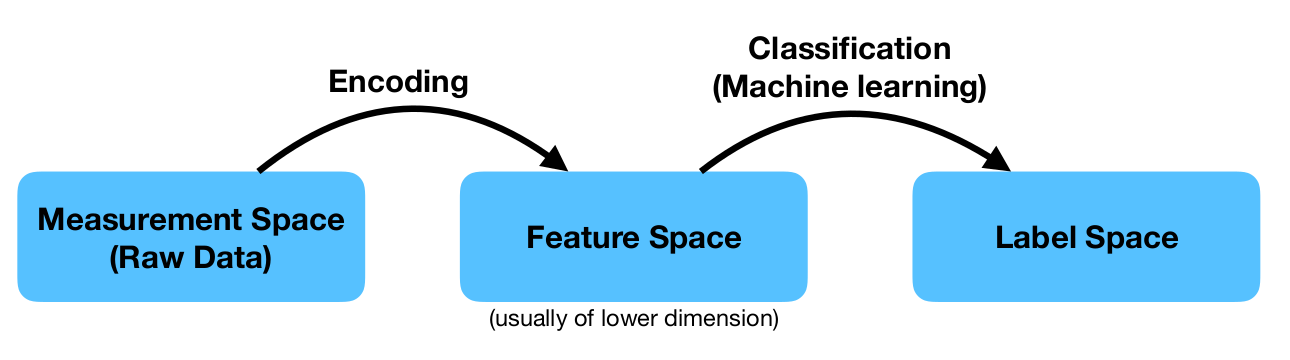
\includegraphics[scale=0.3]{spacesbefore}
  \centering
\end{figure}

\begin{figure}[h]
  \caption{Spaces after the \textit{Deep Learning Era}.}
  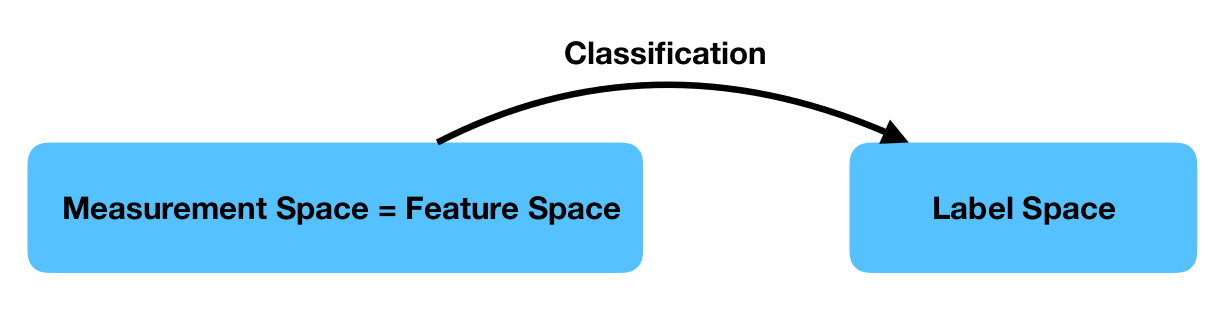
\includegraphics[scale=0.3]{spacesafter}
  \centering
\end{figure}

\subsubsection{Label Space}
There are three main types of \textbf{Label Spaces}:
\begin{itemize}
  \item \textbf{Categorical} (also called class) - $y_i$ is a categorical or nominal variable from some finite set $y_i \in \{1, \ldots, C \}$ (e.g.\ ``Apple'', ``Banana''.).
    The supervised learning task is known as \textbf{classification} or \textbf{pattern recognition}.
  \item \textbf{Real-valued Scalar} - e.g.\ credit score, the task is known as \textbf{regression} or \textbf{function approximation}.
  \item \textbf{Ordinal Regression} - this occurs when the label space has some natural ordering which can be approximated as a regression problem that is subsequently discretised, e.g.\ school grades.
\end{itemize}

\subsection{Unsupervised Learning}
Discovering an underlying, hidden, or latent structure within the data $x$. \\

The aim is to find a structure that explains the data in a more efficient way.
We can think of this as reducing the amount of bits to store the important features of the data, akin to lossy data compression. \\

This is possible in broadly two ways:
\begin{itemize}
  \item \textbf{Dimensionality reduction} - reducing the dimensions in the data.
  \item \textbf{Clustering} - assigning the data to automatically defined categorical labels.
\end{itemize}

\subsection{Reinforcement Learning}
Finding which action to take in order to maximise the received rewards. \\

The main differences are:
\begin{itemize}
  \item The best or correct solution is not given to the agent, only a reward signal.
  \item Feedback is delayed.
  \item Time matters, data is sequential.
  \item Agent's decisions affect the subsequent received data.
\end{itemize}

An example of this is in a moving robot.

\subsection{Main Problems in Machine Learning}
\begin{itemize}
  \item \textbf{Classification} - predicting the right label for an unknown sample.
  \item \textbf{Regression} - approximating an unknown function.
  \item \textbf{Clustering} - grouping data in such a way that data points in the same group (cluster) are more similar to each other than to those in other clusters.
  \item \textbf{Dimensionality Reduction} - reducing the dimensionality of the observed data.
  \item \textbf{Density Estimation} - estimating an unobservable underlying probability density function based on observed data.
  \item \textbf{Policy Search} - finding which action an agent should take, depending on its current state, to maximise the received rewards.
\end{itemize}

\section{Instance Based Learning}

\end{document}
